\lhead{Capítulo \ref{ch_3}}
%\rhead{\newtitle}
\rhead{}
\cfoot{\thepage}
\renewcommand{\headrulewidth}{1pt}
\renewcommand{\footrulewidth}{1pt}
\chapter{Adaptación al Sitio en NOA}\label{ch_3}


En este capítulo se presentan los resultados obtenidos a partir de las distintas evaluaciones realizadas a la AS. 

\section{Medidas en tierra}


Los sitios analizados en esta tesis se resumen en la Tabla \ref{tab:sites}, donde se incluyen sus códigos de identificación, coordenadas geográficas, altitud sobre el nivel del mar, periodos de medición, clasificación climática según Köppen–Geiger \cite{peel2007} y el tipo de piranómetro utilizado. Estas estaciones  están ubicadas en el noroeste de Argentina como puede verse en la Figura \ref{fig:sites} y abarcan diversas condiciones climáticas y geográficas, que van desde tierras bajas subtropicales hasta altiplanos andinos de gran altitud.

\begin{figure}
   \centering
   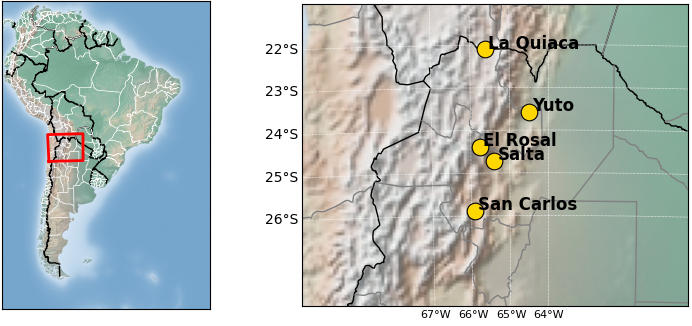
\includegraphics[width=1\linewidth]{figuras/sites.png}
    \caption{Ubicación de la estaciones de medida}
    \label{fig:sites}
\end{figure}


La estación Sa se encuentra en el campus experimental del INENCO, en la Universidad Nacional de Salta. Está situada en un entorno urbano preandino dentro del Valle de Lerma, una zona donde es común la formación de nubes debido a la cercanía de la cordillera. Su clima es subtropical de montaña, con inviernos secos y veranos frescos (Cwb). Las mediciones se realizaron entre 2009 y 2020 utilizando un piranómetro Eppley PSP.\\

La estación Lq, localizada en La Quiaca, presenta un clima estepario frío semiárido (BSk) típico de regiones andinas, y destaca por registrar uno de los mayores niveles de horas de sol anuales en Argentina. Contó con un piranómetro Kipp \& Zonen CMP11 y recopiló datos entre 2021 y 2023.

La estación Yu, ubicada en una zona de clima subtropical húmedo (Cwa), registró datos entre 2017 y 2018 con un sensor CMP11. La estación Sca, también con clima Cwb, operó entre 2012 y 2013 con un piranómetro CMP3. Finalmente, la estación Ero, situada en una región de gran altitud con clima BSk, recopiló datos entre 2016 y 2018, igualmente con un CMP3.

Todas las estaciones utilizan piranómetros que cumplen con los estándares de la norma ISO 9060:2018 Clase A o B para la medición de la irradiancia global horizontal (GHI). Los datos se registraron a intervalos de un minuto, y cada valor corresponde al promedio de seis muestras tomadas cada 10 segundos.




\begin{table}
    \centering
    \renewcommand{\arraystretch}{1.5} % Espaciado vertical en la tabla
    \begin{tabular}{|>{\centering\arraybackslash}p{2cm}|>{\centering\arraybackslash}p{2cm}|>{\centering\arraybackslash}p{2cm}|>{\centering\arraybackslash}p{2cm}|>{\centering\arraybackslash}p{2cm}|>{\centering\arraybackslash}p{2cm}|>{\centering\arraybackslash}p{2cm}|}
        \hline
        \textbf{ID} & \textbf{Provincia} & \textbf{Localidad} & \textbf{Latitud} & \textbf{Longitud}& \textbf{Altitud (m.s.n.m}) & \textbf{Clima}\\ 
        \hline

        \textbf{Yu} & Jujuy & Yuto & -23.58 & -64.5 & 401 & \textbf{Cwa}\\ 
        \textbf{Sa} & Salta & Salta & -24.72 & -65.4 & 1233 & \textbf{Cwb}\\ 
        \textbf{Sca} & Salta & San Carlos & -25.8951 & -65.925 & 1624 & \textbf{Cwb}\\
        \textbf{Er} & Salta & El Rosal & -24.39278 & -65.76806 & 3355& \textbf{Bsk}\\
        \textbf{Lq} & Jujuy & La Quiaca & -24.39278 & -65.76806 & 3355& \textbf{Bsk}\\
        \hline
        
        
    \end{tabular}
    \caption{Estaciones de medidas utilizadas en este trabajo}
    \label{tab:sites}
\end{table}




\subsection{Control de Calidad en las Medidas}

Las medidas fueron sometidas a un control de calidad (QC) siguiendo un procedimiento simplificado basado en \cite{Nollas2023}, con una etapa preliminar de filtrado por inspección visual según las recomendaciones de \cite{abal2020}. Dado que este estudio se basa únicamente en mediciones de irradiancia global horizontal (GHI) y no incluye componentes difusas, se aplicó una versión reducida del procedimiento original. 

La Tabla \ref{tab:qc} resume los filtros utilizados, donde $E$ es la constante solar, $S$ el factor de corrección de la distancia Tierra–Sol, $\theta_z$ el ángulo cenital solar y $kt$ el índice de claridad, definido como la razón entre la GHI y la irradiancia teórica en el tope de la atmósfera sobre un plano horizontal.\\

\begin{table}[h!]
\caption{Filtros de control de calidad aplicados a las mediciones.}
\label{tab:qc}
\centering
\resizebox{\linewidth}{!} {
\def\arraystretch{1.5}
\begin{tabular}{cc}
\hline
\textbf{Filtro} & \textbf{Descripción}\\ 
\hline
F1 & $GHI < 1.5~E~S~(\cos(\theta_z))^{1.2} + 100 \, \text{W/m}^2$  \\
F2 & $GHI > (6.5331 - 0.065502~\theta_z + 1.8312\text{E-4}~\theta_z^2)/(1 + 0.01113~\theta_z)$ \\
F3 & $kt < 1.4$ \& $ (90-\theta_z) < 10^\circ$  \\
\hline
\end{tabular}}
\end{table}

Los filtros aplicados pueden describirse de la siguiente manera:

\begin{itemize}
    \item \textbf{F1}: Rechaza valores que superan un límite físicamente razonable en función de la posición solar.
    \item \textbf{F2}: Descarta mediciones utilizando un umbral empírico dependiente del ángulo cenital.
    \item \textbf{F3}: Elimina valores del índice de claridad superiores a 1.4 cuando el Sol se encuentra a menos de $10^\circ$ sobre el horizonte.
\end{itemize}

El porcentaje de datos diurnos retenidos varió entre estaciones. En particular, el 73\% de los registros de Yu cumplieron los criterios establecidos, frente al 82\% en Sa, 72\% en Sca, aproximadamente 84\% en Ero y 69\% en Lq.





\subsection{Métricas de desempeño}

Los indicadores de desempeño más comunes en el campo de la evaluación del recurso solar han sido abordados por ~\cite{ZHANG}; estos incluyen el Error Medio de Sesgo (MBE), el Error Medio Absoluto (MAE) y el Error Cuadrático Medio (RMSE). Las tres métricas se definen de la siguiente manera:

\begin{equation}
\text{MBE} = \frac{\sum_{i=1}^{n} ( {y_i} - {x_i} ) }{n},
\end{equation}

\begin{equation}
\text{MAE} = \frac{\sum_{i=1}^{n} |{y_i} - {x_i} | }{n},
\end{equation}

\begin{equation}
\text{RMSE} = \sqrt{\frac{1}{n} \sum_{i=1}^{n} \Big({y_i - x_i}\Big)^2},
\label{ec:rrmsd}
\end{equation}

\noindent
donde $x$ y $y$ son los valores medidos y estimados, respectivamente, y $n$ es el tamaño de la muestra. El MBE mide el sesgo sistemático que un modelo puede introducir en una evaluación a largo plazo, mientras que el MAE y el RMSE miden la dispersión del error utilizando normas absolutas y cuadráticas, respectivamente. Debido a su mayor sensibilidad a los valores atípicos, el RMSE se utiliza frecuentemente en esta área. Ambas métricas de dispersión se reportan aquí por completitud. Los tres indicadores se presentan en términos relativos como un porcentaje del promedio de los valores medidos, denominados aquí como MBE (\%), MAE (\%) y RMSE (\%).




\section{Desempeño de los modelos de GHI en el NOA}
Previo a la presentación del desempeño de los distintos procesos de adaptación al sitio se evaluaron los modelos de estimación de GHI disponibles en la región. Siendo este uno de los aportes que se pretende en este trabajo. A continuación se muestran las métricas de desempeño de los modelos calculadas sobre el conjunto de datos de de cada sitio.



% Antes de la tabla, si quieres aumentar la altura de filas
\renewcommand{\arraystretch}{1.5}



\begin{table*}%[]
  \centering
  \caption{Métricas de desempeño (MBE, MAE, RMSE) para cada modelo y conjunto de datos satelitales en los cinco sitios. 
           Los valores están normalizados y expresados como porcentajes relativos al promedio de GHI en cada sitio: 
           396.8~W/m$^{2}$ (Yu), 397~W/m$^{2}$ (Sa), 557.1~W/m$^{2}$ (Sca), 690.6~W/m$^{2}$ (Ero) y 673.7~W/m$^{2}$ (Lq).}
  \resizebox{\linewidth}{!}{%
    \begin{tabular}{|l|ccc|ccc|ccc|ccc|ccc|}
      \hline
      & \multicolumn{3}{c|}{YU} & \multicolumn{3}{c|}{SA} & \multicolumn{3}{c|}{SCA} & \multicolumn{3}{c|}{ERO} & \multicolumn{3}{c|}{LQ} \\
      \cline{2-16}
      Modelo  & MBE & MAE & RMSE & MBE & MAE & RMSE & MBE & MAE & RMSE & MBE & MAE & RMSE & MBE & MAE & RMSE \\
      \hline
      \multicolumn{16}{|c|}{\textit{Resolución Temporal: 15 minutos}} \\
      \hline
      CAMS    & 0.5  & 18.4 & 28.4 & 3.5  & 23.9 & 33.2 & 2.7  & 23   & 30.4 & -23.7& 27.8 & 41.2 &-7.3 & 16.2 & 25.3 \\
      LSA-SAF & 10.7 & 19   & 28.8 & 17.3 & 26.9 & 38.8 & 11.5 & 22.2 & 30.6 & -8.1 & 16.5 & 26.8 & 3.7 & 12.3 & 22.3\\
      \hline
      \multicolumn{16}{|c|}{\textit{Resolución Temporal: horaria}} \\
      \hline
      CAMS    &  0.5 & 16   & 24.1 & 3.6  & 20.5 & 28.8 & 2.9  & 21   & 27.3 & -23.7& 26.8 & 39.5 & -6.1& 14.6 & 22\\
      LSA-SAF & 10.7 & 16.9 & 24.9 & 17.3 & 24.8 & 35   & 11.6 & 20.5 & 27.1 & -8.1 & 15   & 24.3 & 4.6 & 10.9 & 18.7\\
      ERA-5   & -4.2 & 45.4 & 61.9 & 8.5  & 26.8 & 37.5 & 7.4  & 21.2 & 28.9 & -13.7& 19.1 & 25.3 & -1.7& 12   & 19.3\\
      MERRA-2 & 26.9 & 35   & 51.9 & 42.1 & 47   & 63.6 & 12.7 & 21.9 & 29.3 & -3.1 & 13.1 & 20.5 & 1.0 & 13.4 & 21.1\\
      \hline
    \end{tabular}%
  }
\end{table*}
    


\subsection{Análisis de las estimaciones 15-minutales}

La Figura \ref{fig:general-15} muestra la evaluación comparativa de los modelos CAMS y LSA-SAF en los sitios de estudio. En el caso del MBE, se observa que LSA-SAF presenta sesgos positivos en la mayoría de los sitios, indicando una tendencia a la sobreestimación sistemática de las variables simuladas, mientras que CAMS exhibe valores más cercanos a cero o incluso negativos, lo que refleja un comportamiento más balanceado, aunque con subestimaciones marcadas en sitios como Er y Lq.


\begin{figure}
    \centering
    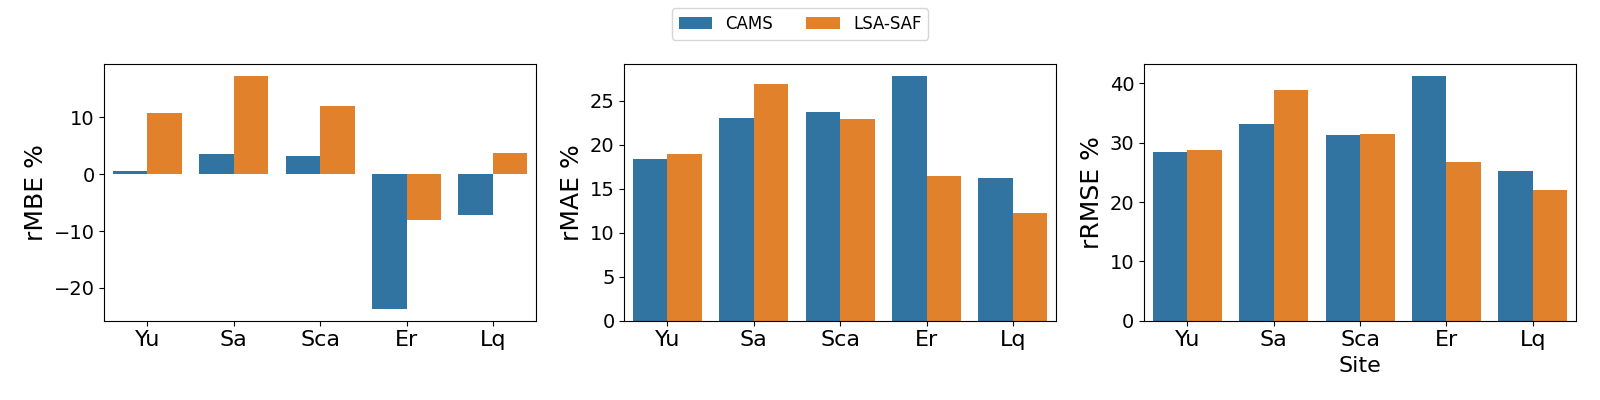
\includegraphics[width=\linewidth]{figuras/errors_15.png}
    \caption{Comparación del desempeño de los modelos CAMS y LSA-SAF en cinco sitios de estudio (Yu, Sa, Sca, Er y Lq) mediante las tres métricas estadísticas: Mean Bias Error (MBE), Mean Absolute Error (MAE) y Root Mean Square Error (RMSE) expresadas en términos relativos a escala 15-minutal.}
    \label{fig:general-15}
\end{figure}

En relación al MAE, ambos modelos presentan magnitudes relativamente similares, aunque LSA-SAF tiende a mostrar errores absolutos ligeramente mayores en sitios como Yu y Sa, mientras que CAMS presenta valores más altos en Sca y Er. Esto sugiere que ninguno de los dos modelos logra una reducción clara y consistente del error en todos los sitios.\\

Por último, en la métrica RMSE, que penaliza los errores grandes, se mantiene un patrón semejante: LSA-SAF suele exhibir errores algo superiores a los de CAMS en Yu y Sa, mientras que en Er y Lq la diferencia favorece al modelo satelital. En general, los resultados muestran que el desempeño relativo de los modelos depende fuertemente del sitio, sin que exista un claro ganador en todos los casos.\\


\begin{figure} 
\centering 
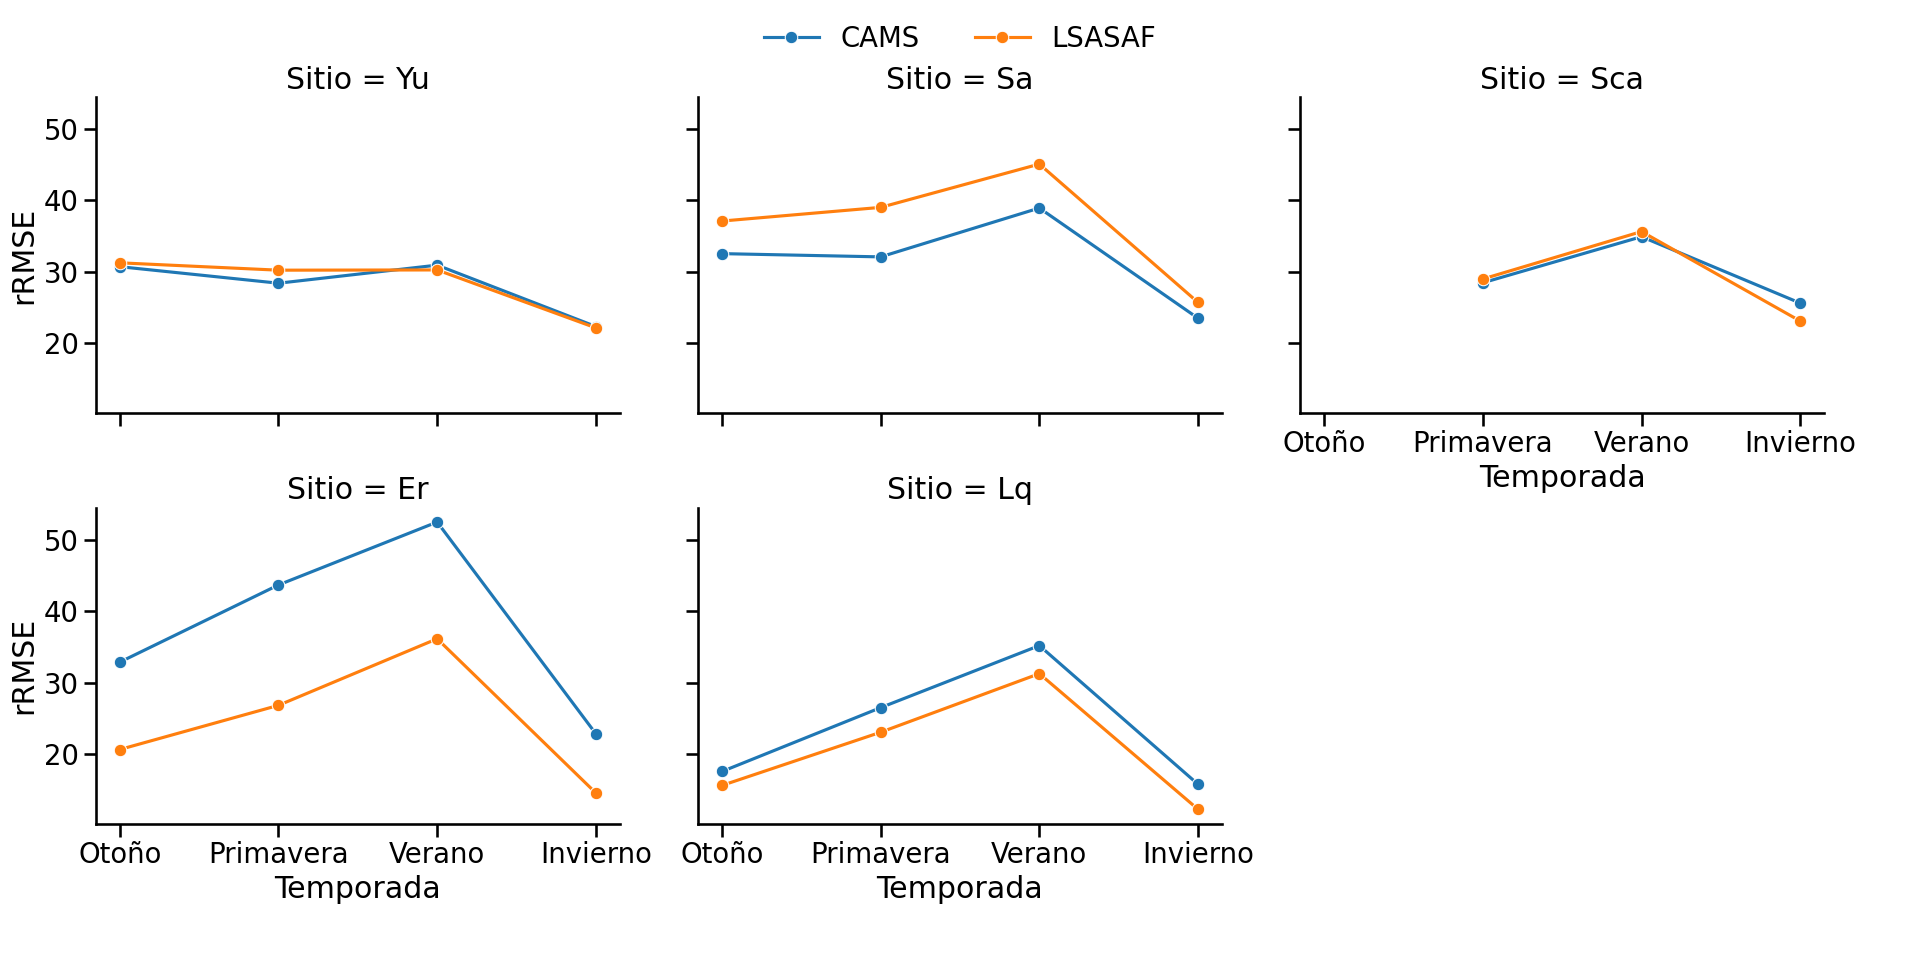
\includegraphics[width=\linewidth]{figuras/season_15_tesis.png}
 \caption{Figura \ref{fig:season-15}. Variación estacional del rRMSE (\%) para los productos CAMS y LSA-SAF con resolución de 15 minutos en todos los sitios de estudio. Se evidencia un aumento del error durante el verano en la mayoría de los sitios, mientras que en Yuto el rRMSE se mantiene estable, sugiriendo que la presencia de nubosidad estacional afecta de manera diferenciada la precisión de las estimaciones de radiación solar.} 
\label{fig:season-15} 
\end{figure}


La Figura \ref{fig:season-15} muestra la variación estacional del rRMSE (\%) para los productos CAMS y LSA-SAF con resolución de 15 minutos en todos los sitios de estudio. Se observa una clara tendencia estacional en el comportamiento del error: en general, el rRMSE tiende a aumentar durante el verano, lo que indica que la precisión de las estimaciones disminuye en este período en la mayoría de los sitios. La excepción es Yuto, donde el error permanece relativamente estable a lo largo de las estaciones. Este patrón sugiere que durante el verano hay una mayor presencia de nubosidad, lo cual podría estar afectando la capacidad de los modelos satelitales para estimar correctamente la radiación solar, mientras que en otras estaciones la cobertura nubosa es menor, permitiendo estimaciones más precisas.







\begin{figure}
    \centering
    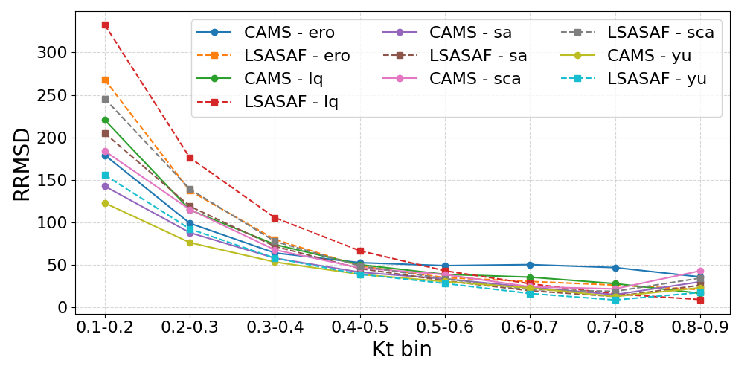
\includegraphics[width=\linewidth]{figuras/RMSE-kt-15.pdf}
    \caption{Variación del error cuadrático medio relativo (RRMSD) en función del indice de claridad (kt) para los cinco sitios analizados (YU, SA, SCA, ERO y LQ). Resultados para CAMS (líneas continuas) y LSASAF (líneas punteadas).}
    \label{fig:RMSE-kt-15}
\end{figure}



En el caso de RRMSD vs Kt (Figura \ref{fig:RMSE-kt-15}), se observa una marcada disminución del error a medida que aumenta la claridad atmosférica. Para condiciones de cielo más nuboso (Kt < 0.3), los valores de RRMSD son elevados en todos los sitios, superando en algunos casos los 200 \%, especialmente en la estimación proveniente de LSASAF. Sin embargo, conforme Kt aumenta (>0.5), el error desciende rápidamente y tiende a estabilizarse por debajo del 50\%, alcanzando valores mínimos en condiciones de cielo despejado (Kt > 0.7). Esta tendencia se mantiene consistente en ambos productos (CAMS y LSASAF), aunque LSASAF presenta errores relativamente mayores en las condiciones más turbias.




\begin{figure}
    \centering
    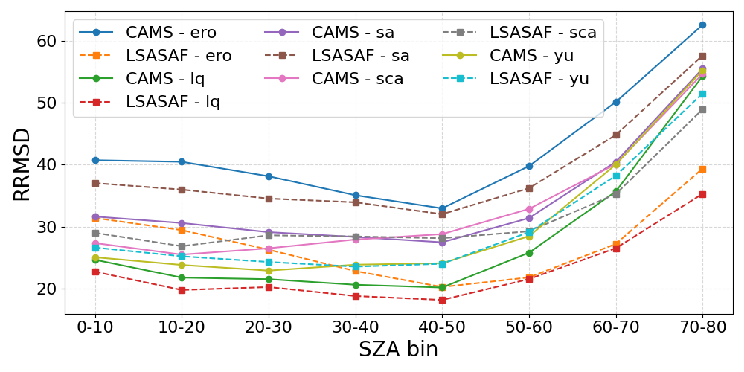
\includegraphics[width=0.8\textwidth]{figuras/RMSE-sza-15.pdf}
    \caption{Variación del error cuadrático medio relativo (RRMSD) en función del ángulo cenital solar (SZA) para los cinco sitios analizados (YU, SA, SCA, ERO y LQ). Resultados para CAMS (líneas continuas) y LSASAF (líneas punteadas).}
    \label{fig:RMSE-SZA-15}
\end{figure}



Por otro lado, la relación RRMSD vs SZA (Figura \ref{fig:RMSE-SZA-15}) evidencia un comportamiento en forma de “U” invertida: los menores errores se concentran en ángulos intermedios (30°–50°), mientras que hacia ángulos bajos (<20°) y altos (>70°) el error aumenta de manera significativa. Esta tendencia se observa en los cinco sitios, con un incremento más pronunciado en ERO y SA en las condiciones de SZA más extremas. En general, CAMS muestra un mejor desempeño que LSASAF en la mayoría de los intervalos, aunque las diferencias se reducen en los ángulos medios.

En conjunto, estos resultados indican que la precisión de ambos productos depende fuertemente de las condiciones atmosféricas (Kt) y de la geometría solar (SZA). En cielos despejados y ángulos intermedios, los errores se reducen notablemente, mientras que en condiciones nubosas y en situaciones de baja o alta elevación solar los modelos presentan las mayores limitaciones.


\subsection{Análisis de las estimaciones horarias}



\subsection{División del conjunto de datos}
De acuerdo a lo indicado en la sección \ref{MLM} el conjunto de datos debe ser segmentado con fin de evaluar el rendimiento de los modelos de aprendizaje automático utilizados en la regresión del proceso de adaptación al sitio y controlar el sobre-entrenamiento de los modelos. En el contexto de AS en los trabajos \cite{POLO2016, POLO2020} se recomienda tomar al menos un año de medidas para la calibración de los modelos. Siguiendo estas ideas el conjunto de medidas fue dividido en subconjunto de entrenamiento, validación y prueba.  


\begin{table}[ht]
    \centering
    \renewcommand{\arraystretch}{1.5} % Espaciado vertical en la tabla
    \begin{tabular}{|>{\centering\arraybackslash}p{2cm}|>{\centering\arraybackslash}p{3cm}|>{\centering\arraybackslash}p{3cm}|>{\centering\arraybackslash}p{4cm}|}
        \hline
        \textbf{ID} & \textbf{Entrenamiento} & \textbf{Validación} & \textbf{Prueba}\\ 
        \hline

        \textbf{YU}  & 2017 & 2017 & 2018 \\ 
        \textbf{SA}  & 2009 & 2009 & 2010 - 2024 \\ 
        \textbf{SCA} & 2013 & 2013 & 2012-2014 \\
        \textbf{ERO} & 2013 & 2013 & 2014 - 2024  \\
        \textbf{LQ}  & 2020 & 2020 & 2021 - 2024  \\
    \hline
    \end{tabular}
    \caption{División del conjunto de datos en entrenamiento, validación y prueba }
    \label{tab:tvt}
\end{table}

    



\begin{table*}%[]
  \centering
  \label{tbl:metrics_test}
  \caption{Métricas de desempeño (MBE, MAE, RMSE) para cada modelo y conjunto de datos satelitales en los cinco sitios en el \textbf{conjunto de pruebas}. 
           Los valores están normalizados y expresados como porcentajes relativos al promedio de GHI en cada sitio: 
           396.8~W/m$^{2}$ (Yu), 397~W/m$^{2}$ (Sa), 557.1~W/m$^{2}$ (Sca), 690.6~W/m$^{2}$ (Ero) y 673.7~W/m$^{2}$ (Lq).}
  \resizebox{\linewidth}{!}{%
    \begin{tabular}{|l|ccc|ccc|ccc|ccc|ccc|}
      \hline
      & \multicolumn{3}{c|}{YU} & \multicolumn{3}{c|}{SA} & \multicolumn{3}{c|}{SCA} & \multicolumn{3}{c|}{ERO} & \multicolumn{3}{c|}{LQ} \\
      \cline{2-16}
      Modelo  & MBE & MAE & RMSE & MBE & MAE & RMSE & MBE & MAE & RMSE & MBE & MAE & RMSE & MBE & MAE & RMSE \\
      \hline
      \multicolumn{16}{|c|}{\textit{Resolución Temporal: 15 minutos}} \\
      \hline
      CAMS    & -0.2 & 17.4 & 27.2 & 3.9  & 23.4 & 33.7 & 2.6  & 21.8 & 29.8 & -23.6 & 27.6 & 40.9 & -6.9 & 16.5 & 25.8 \\
      LSA-SAF & 7.6  & 16.5 & 25.5 & 17.9 & 27.4 & 39.4 & 13.1 & 22.2 & 30.9 & -7.7  & 16.2 & 26.5 & 4.0  & 12.6 & 22.6 \\
      \hline
      \multicolumn{16}{|c|}{\textit{Resolución Temporal: horaria}} \\
      \hline
      CAMS    & -0.2 & 15.3 & 23.5 & 4.0 & 20.9 & 29.3 & 3.0 & 19.7 & 26.1 & -23.6 & 26.6 & 39.3 & -4.8 & 14.5 & 21.6 \\
      LSA-SAF & 7.6  & 14.5 & 21.9 & 17.9 & 25.3 & 35.7 & 13.3 & 20.3 & 27.1 & -7.7  & 14.8 & 24.0 & 4.8  & 10.9 & 18.2 \\
      ERA-5   & -4.0 & 43.5 & 60.2 & 9.4  & 27.1 & 37.7 & 1.9  & 20.2 & 29.7 & -14.0 & 19.3 & 25.6 & -0.8 & 11.3 & 18.4 \\
      MERRA-2 & 25.0 & 33.6 & 51.2 & 43.4 & 48.3 & 65.0 & 10.9 & 21.7 & 30.3 & -3.8  & 13.1 & 20.4 & 1.4  & 13.4 & 20.8 \\
      \hline
    \end{tabular}%
  }
\end{table*}

    



\section{Adaptación al sitio con una variable descriptiva}







En los trabajos citados en las secciones anteriores sobre la evaluación del proceso de Adaptación al Sitio (AS), se ha prestado escasa atención a las razones subyacentes por las cuales ciertos modelos de ML superan a otros en dicho proceso. Considerando que algunos modelos de ML presentan una naturaleza inherentemente más compleja que otros, podría pensarse que modelos más complejos ofrecerían un mejor rendimiento en comparación con aquellos de menor complejidad. En este contexto, el término complejidad hace referencia tanto a la complejidad computacional —es decir, la cantidad de operaciones necesarias para ejecutar el modelo— como a la complejidad conceptual asociada al nivel de conocimiento requerido para comprender su funcionamiento.\\

En esta sección, se presenta una implementación del proceso de AS basada en uno de los enfoques clásicos, el cual consiste en adaptar una serie temporal modelada (proveniente de datos satelitales o de reanálisis) utilizando como referencia una serie de mediciones in situ.\\

Dado que el modelo de Regresión Lineal Simple (RLS) puede considerarse el menos complejo entre los modelos empleados en este estudio, la primera evaluación del proceso de SA en la región de interés se realiza utilizando dicho modelo. El objetivo es comparar el desempeño de la RLS con el de otros modelos de regresión más complejos, tales como Perceptrón Multicapa (MLP) y XGBoost, utilizando las mismas métricas de evaluación.\\


Para ambos modelos, MLP y XGBoost, determinar la configuración óptima de hiperparámetros fue esencial para lograr un desempeño consistente a través de las particiones de validación cruzada. Esto se llevó a cabo mediante una búsqueda exhaustiva en rejilla implementada con la función \textbf{GridSearchCV} de la biblioteca \textbf{Scikit-learn} en Python \cite{Pedregosa2012}. Los rangos específicos de hiperparámetros evaluados para los modelos MLP y XGB se describen en la Tabla \ref{tab:gridsearch}. La selección de hiperparámetros óptimos es un paso crítico en el aprendizaje automático, ya que influyen directamente en la complejidad del modelo, su capacidad de generalización y su rendimiento predictivo global \cite{Goodfellow2016}.

\begin{table}[ht!]
\caption{Espacio cartesiano de hiperparámetros para las técnicas de aprendizaje supervisado.}
\label{tab:gridsearch}
\centering
\resizebox{\linewidth}{!} {
\def\arraystretch{1.5}
\begin{tabular}{lcccc}
\hline
\textbf{Hiperparámetro} & \textbf{Inferior} & \textbf{Superior} & \textbf{Paso} & \textbf{Función de transformación} \\
\hline
MLP\\
\hline
 Capas ocultas        & 1    & 3     & 1   & - \\
 Nodos ocultos        & 1    & 4     & 1   & $2^{x}$ \\
 Fracción de dropout  & 0    & 0.3   & 0.1 & - \\
 Tasa de aprendizaje  & -3   & -1    & 1   & $10^{x}$ \\
\hline
XGBoost\\
\hline
Booster               & gbtree & & & \\
 Estimadores          & 1    & 50    & 10  & - \\
 Profundidad máxima   & 2    & 5     & 1   & $2^{x}$ \\
 Tasa de aprendizaje  & -3   & -1    & 1   & $10^{x}$ \\
\hline
\end{tabular}}
\end{table}

En cuanto al preprocesamiento de los datos de entrada, la normalización o el escalado de características es una práctica común en aprendizaje automático para mejorar la convergencia y la estabilidad, particularmente en modelos sensibles a la magnitud de las variables de entrada. Sin embargo, en este estudio \textbf{no se aplicó normalización}, ya que no se consideró necesaria para los modelos y datos utilizados.  

En el caso del modelo \textbf{SLR}, el escalado de la variable independiente no es necesario porque el modelo es inherentemente invariante al escalado: multiplicar la entrada por un factor constante provoca un cambio inversamente proporcional en el coeficiente de la pendiente, dejando las predicciones sin alterar.  

De manera similar, \textbf{XGB}, cuando se implementa con árboles de decisión como aprendices base, \textbf{no requiere escalado de características}, ya que las divisiones en los nodos dependen del \textbf{orden relativo} de los valores y no de sus magnitudes absolutas \cite{Soria2022, Chen2016}.  

En el caso del modelo \textbf{MLP}, el escalado puede ser importante cuando las variables de entrada difieren significativamente en su rango o unidades. Sin embargo, en el presente estudio se utilizó \textbf{una sola variable de entrada} (GHI derivado de satélite), expresada en las \textbf{mismas unidades y rango} que la variable objetivo (GHI medido en superficie). Por lo tanto, no se consideró necesaria ninguna normalización adicional.

Los resultados obtenidos son expresados en la Tabla \ref{tab:metrics-as-1}.


\begin{table*}%[]
  \centering
  \label{tab:metrics-as-1}
  \caption{Métricas de desempeño (MBE, MAE, RMSE) para cada modelo adaptado en los cinco sitios en el \textbf{conjunto de pruebas}}
  \resizebox{\linewidth}{!}{%
    \begin{tabular}{|l|ccc|ccc|ccc|ccc|ccc|}
      \hline
      & \multicolumn{3}{c|}{YU} & \multicolumn{3}{c|}{SA} & \multicolumn{3}{c|}{SCA} & \multicolumn{3}{c|}{ERO} & \multicolumn{3}{c|}{LQ} \\
      \cline{2-16}
      Modelo  & MBE & MAE & RMSE & MBE & MAE & RMSE & MBE & MAE & RMSE & MBE & MAE & RMSE & MBE & MAE & RMSE \\
      \hline
      \multicolumn{16}{|c|}{\textit{Resolución Temporal: 15 minutos}} \\
      \hline
      CAMS SLR    & -0.9 & 17.1 & 26.4 &  3.8 & 21.3 & 31.5 & -1.5 & 18.4 & 26.0 &  2.5 & 24.8 & 31.5 &  2.1 & 15.9 & 23.5 \\
      CAMS MLP    & -4.4 & 17.7 & 26.2 &  4.8 & 21.4 & 31.6 &  7.7 & 17.8 & 27.7 &  0.5 & 24.1 & 31.2 &  9.1 & 19.4 & 25.6 \\
      CAMS XGB    & -1.3 & 17.1 & 26.0 &  3.8 & 21.4 & 31.4 & -1.8 & 18.9 & 26.2 &  2.5 & 23.9 & 30.9 &  2.2 & 15.9 & 23.5 \\
      \hline
      LSASAF SLR  & -5.5 & 18.4 & 25.0 &  4.4 & 23.9 & 34.6 &  1.0 & 18.0 & 26.7 &  2.7 & 17.1 & 25.4 &  2.2 & 12.9 & 22.3 \\
      LSASAF MLP  & -7.1 & 18.6 & 25.0 &  4.5 & 23.6 & 34.5 &  5.9 & 18.4 & 26.6 &  2.5 & 17.0 & 25.3 & -0.4 & 13.6 & 22.1 \\    
      LSASAF XGB  & -6.0 & 18.2 & 24.9 &  4.3 & 23.9 & 34.6 &  0.5 & 18.6 & 27.0 &  2.4 & 17.2 & 25.1 &  2.3 & 13.1 & 22.3 \\
      \hline
      \multicolumn{16}{|c|}{\textit{Resolución Temporal: horaria}} \\
      \hline
      CAMS SLR    & -1.3 & 14.7 & 22.7 &  3.5 & 18.5 & 27.0 & -1.7 & 15.9 & 22.0 &  2.1 & 23.4 & 29.6 &  2.6 & 13.8 & 19.4 \\
      LSASAF SLR  & -5.5 & 16.0 & 21.2 &  4.3 & 21.2 & 30.5 &  1.1 & 15.6 & 22.7 &  2.5 & 15.7 & 22.8 &  0.3 & 10.6 & 17.4 \\
      ERA-5 SLR   &  1.2 & 44.0 & 55.1 &  6.4 & 26.5 & 36.9 & -6.4 & 20.1 & 29.1 & -0.6 & 15.4 & 21.4 &  2.1 & 11.6 & 18.4 \\
      MERRA-2 SLR & -3.6 & 34.7 & 44.1 &  7.1 & 35.2 & 46.0 & -2.2 & 20.3 & 27.7 &  0.7 & 12.9 & 20.1 &  0.3 & 13.1 & 20.4 \\
      \hline
      CAMS MLP    & -4.9 & 16.2 & 23.0 &  4.3 & 18.6 & 27.2 & -4.0 & 16.6 & 22.4 &  3.8 & 23.5 & 29.5 & -0.5 & 13.0 & 19.2 \\
      LSASAF MLP  & -5.4 & 15.4 & 20.9 &  2.5 & 21.4 & 30.2 &  8.3 & 16.1 & 24.1 &  9.6 & 19.4 & 24.6 & -3.8 & 12.1 & 17.8 \\
      ERA-5 MLP   &  0.2 & 43.7 & 55.1 &  9.6 & 27.1 & 37.6 & -1.8 & 19.0 & 28.5 & -7.5 & 16.7 & 23.1 &  0.1 & 11.3 & 18.3 \\
      MERRA-2 MLP &  0.7 & 33.7 & 43.9 &  0.8 & 36.3 & 45.4 & -0.3 & 19.5 & 27.5 & 11.7 & 17.5 & 23.4 & -2.8 & 13.4 & 20.6 \\
      \hline
      CAMS XGB    & -1.6 & 14.8 & 22.2 &  3.4 & 18.9 & 27.1 & -2.4 & 16.6 & 22.4 &  2.1 & 22.8 & 29.2 &  2.7 & 13.9 & 19.6 \\
      LSASAF XGB  & -6.1 & 16.0 & 21.3 &  4.1 & 21.4 & 30.6 &  0.0 & 16.9 & 23.4 &  2.2 & 15.9 & 22.6 &  0.2 & 10.9 & 17.4 \\
      ERA-5 XGB   &  1.4 & 44.6 & 55.4 &  6.3 & 27.3 & 37.4 & -7.3 & 20.7 & 29.3 & -0.5 & 15.2 & 21.2 &  2.0 & 11.8 & 18.6 \\
      MERRA-2 XGB & -4.9 & 35.3 & 44.5 &  6.9 & 35.6 & 46.1 & -2.8 & 20.8 & 28.2 &  0.8 & 13.3 & 20.3 &  0.2 & 13.5 & 20.6 \\
      \hline
    \end{tabular}%
  }
\end{table*}

La evaluación comparativa de los modelos SLR,MLP y XGB, utilizando como variables de entrada los productos satelitales \textit{CAMS} y \textit{LSA-SAF}, se realizó en cinco sitios con características climáticas y geográficas diversas. El desempeño se expresó en términos de error medio de sesgo (MBE), error absoluto medio (MAE) y raíz del error cuadrático medio (RMSE), todos normalizados respecto al promedio de la irradiancia global horizontal (GHI) en cada estación (Tablas~\ref{tab:metrics-as-1} y \ref{tbl:metrics_test}).  

En términos generales, los errores normalizados se mantuvieron dentro de un rango moderado en todas las combinaciones de modelos y conjuntos de datos, sin observarse diferencias sustanciales entre los enfoques lineales y los no lineales. El modelo RLS mostró un desempeño competitivo en ambos conjuntos de datos, con métricas de error cercanas a las obtenidas por los modelos más complejos.  

En el caso de \textbf{CAMS}, aunque el MLP logró reducir ligeramente el RMSE en algunos sitios, esto se produjo a costa de sesgos más pronunciados en el MBE, lo cual evidencia una compensación entre reducción de varianza e incremento del error sistemático. El modelo XGB, por su parte, presentó un comportamiento muy similar al de RLS, con diferencias marginales.  

Por otro lado, al emplear \textbf{LSA-SAF} se observó una ligera mejora respecto a CAMS, particularmente en estaciones de mayor altitud (ERO y LQ), donde tanto XGB como MLP alcanzaron menores valores de MAE y RMSE. Esto sugiere que la mayor resolución temporal o la representación más detallada de nubes en LSA-SAF aportan información adicional útil para el proceso de adaptación local.  

No obstante, el incremento de la complejidad del modelo no se tradujo en ganancias sustanciales de desempeño. Estos resultados indican que, dadas las condiciones actuales de calidad de los datos satelitales, los modelos simples como RLS son capaces de capturar gran parte de la relación entre los insumos derivados de satélite y las mediciones de GHI en superficie, ofreciendo además mayor robustez frente al ruido y a las limitaciones en los datos de entrenamiento.  

\begin{figure}[ht]
\centering
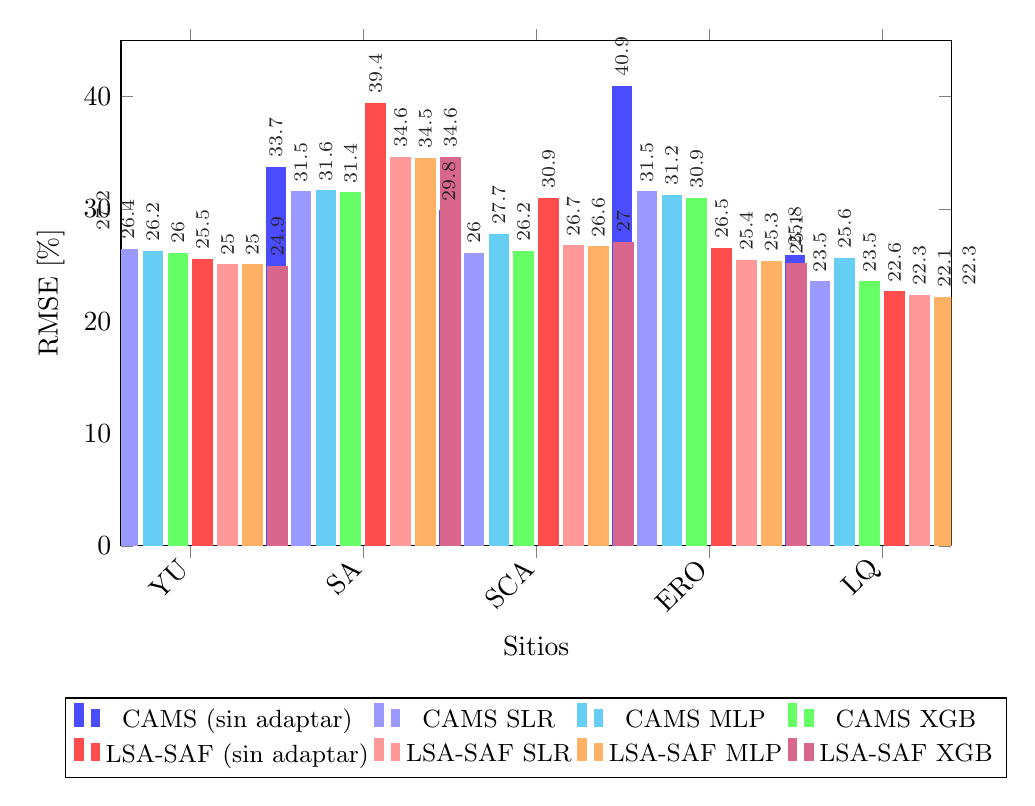
\begin{tikzpicture}
\begin{axis}[
    ybar,
    bar width=7pt,
    width=\linewidth,
    height=8cm,
    ylabel={RMSE [\%]},
    xlabel={Sitios},
    symbolic x coords={YU, SA, SCA, ERO, LQ},
    xtick=data,
    xticklabel style={rotate=45, anchor=east},
    enlarge x limits=0.1,
    ymin=0,
    nodes near coords,
    nodes near coords style={font=\scriptsize, rotate=90, anchor=west, text=black!85},
    legend style={at={(0.5,-0.30)}, anchor=north, legend columns=4, font=\small},
    cycle list={{blue!70},{blue!40},{cyan!60},{green!60},{red!70},{red!40},{orange!60},{purple!60}}
]

% ---- CAMS sin adaptar ----
\addplot+[fill=blue!70] coordinates {(YU,27.2) (SA,33.7) (SCA,29.8) (ERO,40.9) (LQ,25.8)};

% ---- CAMS adaptados ----
\addplot+[fill=blue!40] coordinates {(YU,26.4) (SA,31.5) (SCA,26.0) (ERO,31.5) (LQ,23.5)}; % SLR
\addplot+[fill=cyan!60] coordinates {(YU,26.2) (SA,31.6) (SCA,27.7) (ERO,31.2) (LQ,25.6)}; % MLP
\addplot+[fill=green!60] coordinates {(YU,26.0) (SA,31.4) (SCA,26.2) (ERO,30.9) (LQ,23.5)}; % XGB

% ---- LSA-SAF sin adaptar ----
\addplot+[fill=red!70] coordinates {(YU,25.5) (SA,39.4) (SCA,30.9) (ERO,26.5) (LQ,22.6)};

% ---- LSA-SAF adaptados ----
\addplot+[fill=red!40] coordinates {(YU,25.0) (SA,34.6) (SCA,26.7) (ERO,25.4) (LQ,22.3)}; % SLR
\addplot+[fill=orange!60] coordinates {(YU,25.0) (SA,34.5) (SCA,26.6) (ERO,25.3) (LQ,22.1)}; % MLP
\addplot+[fill=purple!60] coordinates {(YU,24.9) (SA,34.6) (SCA,27.0) (ERO,25.1) (LQ,22.3)}; % XGB

\legend{CAMS (sin adaptar), CAMS SLR, CAMS MLP, CAMS XGB, 
        LSA-SAF (sin adaptar), LSA-SAF SLR, LSA-SAF MLP, LSA-SAF XGB}
\end{axis}
\end{tikzpicture}
\caption{RMSE en resolución de 15 minutos para cada modelo y sitio, comparando modelos sin adaptación y adaptados.}
\label{fig:rmse15}
\end{figure}

La Figura \ref{fig:rmse15} muestra el comportamiento del RMSE (\%) en cada sitio para los diferentes modelos de regresión utilizados. Se observa que todas las propuestas de adaptación logran reducir el RMSE en cada sitio. Aunque en algunos casos la mejora puede ser modesta, como en YU y LQ, queda evidenciado que un simple ajuste específico puede mejorar el desempeño del modelo para una ubicación determinada.

Además, los resultados de la adaptación dependen del modelo de estimación empleado. Cada modelo impone un límite sobre la precisión de la serie resultante, y optimizar su salida no garantiza necesariamente un desempeño superior frente a otro modelo que, de forma natural, ya proporciona una estimación más adecuada para un sitio específico.\\





\begin{figure}
    \centering
    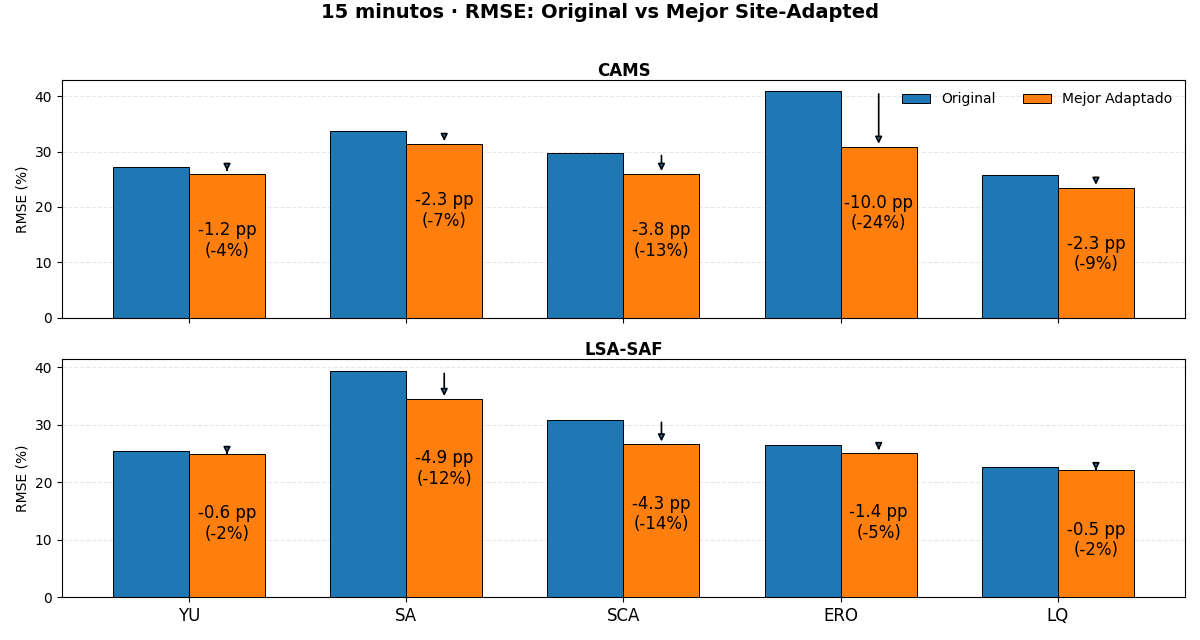
\includegraphics[width=0.9\textwidth]{figuras/comparativasRMSE15.png}
    \caption{Variación del error cuadrático medio relativo (RRMSD) en función del ángulo cenital solar (SZA) para los cinco sitios analizados (YU, SA, SCA, ERO y LQ). Resultados para CAMS (líneas continuas) y LSASAF (líneas punteadas).}
    \label{fig:RMSE-15}
\end{figure}



%\begin{figure}
%    \centering
%    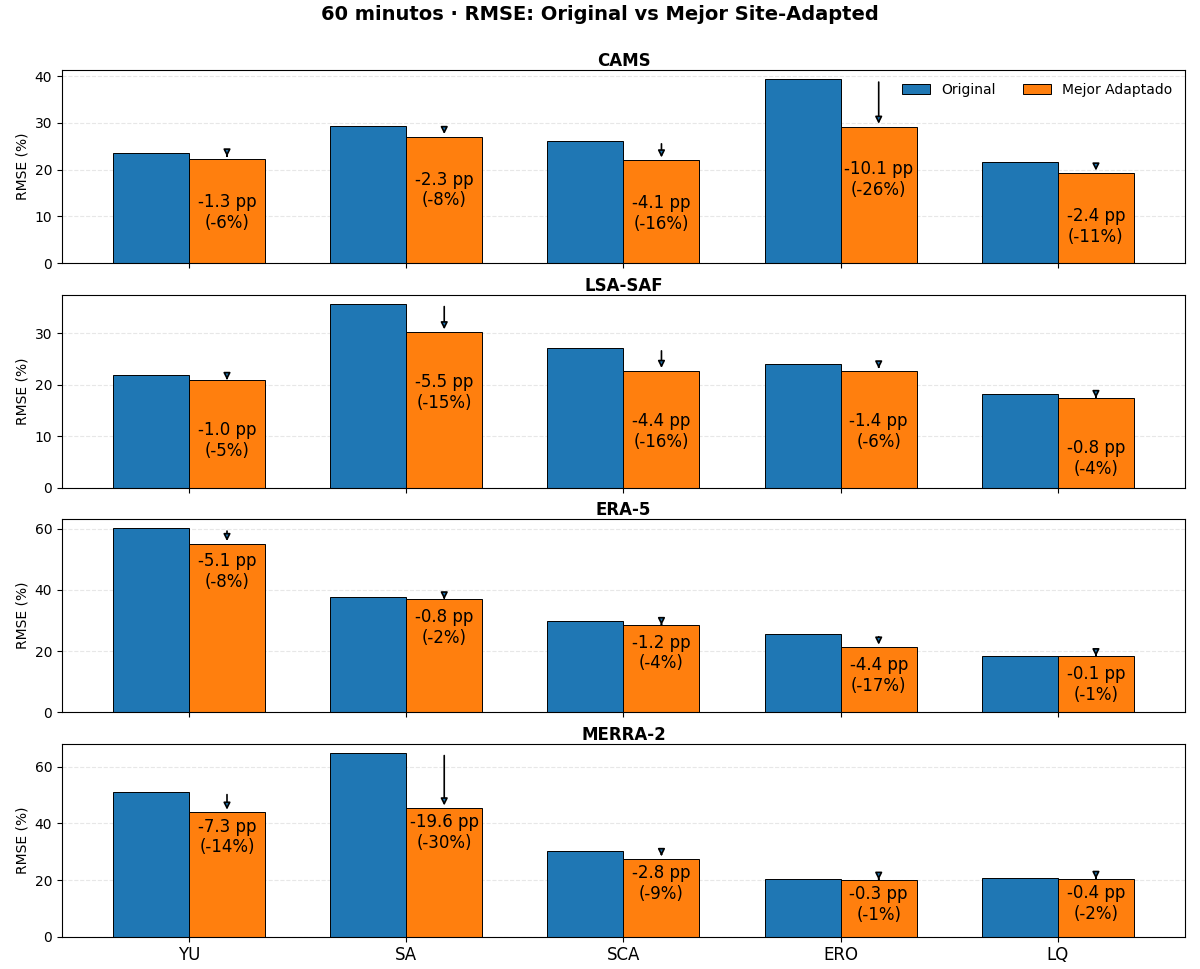
\includegraphics[width=0.9\textwidth]{figuras/comparativasRMSE60.png}
%    \caption{Variación del error cuadrático medio relativo (RRMSD) en función del ángulo cenital solar (SZA) para los cinco sitios analizados (YU, SA, SCA, ERO y LQ). Resultados para CAMS (líneas continuas) y LSASAF (líneas punteadas).}
%    \label{fig:RMSE-60}
%\end{figure}


Los hallazgos de este primer estudio indican que, en el contexto de la adaptación del sitio para GHI utilizando productos derivados de satélite como CAMS y LSA-SAF, los modelos de aprendizaje automático evaluados SLR, XGB y MLP mostraron un rendimiento comparable en términos de métricas de error estándar, con diferencias mínimas entre ellos. A pesar de su simplicidad, SLR demostró una notable capacidad para capturar la relación entre los datos derivados de satélite y las mediciones terrestres, logrando niveles de error relativo similares a los obtenidos por los modelos XGB y MLP, más complejos.
Estos resultados sugieren que la calidad de los datos de entrada impone un límite superior a las mejoras de precisión alcanzables que ofrecen los modelos complejos. Los productos satelitales empleados presentan incertidumbres inherentes y carecen de la resolución necesaria para considerar fenómenos localizados de alta frecuencia, como los efectos microclimáticos o la variabilidad inducida por el terreno. En consecuencia, aumentar la complejidad del modelo no mejora sustancialmente el rendimiento predictivo en estas condiciones de datos. En este sentido, la capacidad predictiva de los modelos complejos se vuelve redundante cuando la relación subyacente entre las variables es predominantemente lineal o solo ligeramente no lineal, lo que explica el excelente rendimiento del SLR.
Además, el análisis reveló que los modelos más flexibles, como el MLP, son propensos al sobreajuste, lo que genera un comportamiento inconsistente en diferentes métricas de rendimiento. Esto subraya la importancia de equilibrar la complejidad del modelo con la calidad de los datos para evitar comprometer la capacidad de generalización del modelo. En resumen, dada la calidad actual de los datos y las características del sitio, modelos simples como el SLR representan una solución robusta, interpretable y computacionalmente eficiente para la estimación del GHI adaptada al sitio. Es más probable lograr mejoras significativas en la precisión de la estimación incorporando variables meteorológicas adicionales, aplicando técnicas de descomposición temporal o desarrollando enfoques híbridos que combinen modelos físicos con correcciones estadísticas, en lugar de simplemente aumentar la complejidad de los algoritmos de aprendizaje automático.

 


\section{Adaptación al sitio con múltiples variables descriptivas}

Los modelos de aprendizaje automático se emplean cada vez más para identificar patrones y extraer información significativa de grandes volúmenes de datos. No obstante, la efectividad de estos modelos depende en gran medida de la calidad de las características utilizadas durante el entrenamiento. La \textbf{selección de características}, un paso crucial en el preprocesamiento de datos, consiste en identificar las variables más relevantes y eliminar aquellas que sean redundantes o irrelevantes \cite{liu2023, Huang2024}. Este proceso no solo incrementa la interpretabilidad del modelo, sino que también mejora su eficiencia computacional y su capacidad predictiva. Un exceso de características o la inclusión de variables irrelevantes puede causar \textbf{sobreajuste}, donde el modelo presenta un buen desempeño con los datos de entrenamiento pero falla al generalizar a datos no vistos \cite{che2024a}. La selección de características ayuda a mitigar este problema al reducir la dimensionalidad, fomentando la creación de modelos más robustos y generalizables. Además, contribuye a disminuir los costos computacionales y el tiempo requerido para entrenar el modelo, consolidándose como una herramienta esencial tanto para investigadores como para profesionales \cite{Cheng2024}.\\

Las técnicas de selección de características se agrupan en tres categorías principales: \textbf{métodos de filtro, métodos envolventes y métodos embebidos}, cada uno con su propia metodología, ventajas y limitaciones:  

\paragraph{Métodos de filtro.} Los métodos de filtro evalúan la relevancia de cada característica mediante criterios estadísticos como correlación, información mutua o varianza. Son computacionalmente eficientes y no dependen de un algoritmo de aprendizaje específico. Sin embargo, pueden no captar las interacciones entre variables. Ejemplos comunes incluyen la correlación de Pearson, las pruebas chi-cuadrado y la ganancia de información.  

\paragraph{Métodos envolventes.} Estos métodos consisten en entrenar y evaluar un modelo de aprendizaje automático múltiples veces para identificar el subconjunto óptimo de características. Técnicas como la selección hacia adelante, la eliminación hacia atrás y la eliminación recursiva de características (RFE) son ejemplos típicos \cite{Che2024b,liu2024}. Aunque suelen proporcionar mayor precisión, son costosos en términos computacionales y pueden no escalar eficientemente con conjuntos de datos grandes.  

\paragraph{Métodos embebidos.} Los métodos embebidos incorporan la selección de características directamente en el proceso de entrenamiento del modelo. Ejemplos incluyen técnicas de regularización como LASSO (regularización L1) y modelos basados en árboles de decisión. Este enfoque logra un equilibrio entre eficiencia y rendimiento, convirtiéndolo en una opción ampliamente utilizada en distintas aplicaciones. \\

Comprender estas técnicas permite a los profesionales seleccionar el método más adecuado según las características del conjunto de datos, el dominio del problema y las limitaciones computacionales.\\

En esta sección se documentan los resultados obtenidos al seleccionar tres métodos complementarios para la selección de variables con el objetivo de identificar los mejores regresores que contribuyan a la mejora de la estimación de la GHI en el contexto de la adaptación al sitio: RFE, LASSO y Stepwise.  

\paragraph{Eliminación recursiva de características (RFE).} RFE permite evaluar de manera iterativa la importancia de cada variable en el modelo, eliminando progresivamente las menos relevantes. Este enfoque es particularmente útil en el análisis de variables de geometría solar, donde pueden existir correlaciones complejas entre diferentes parámetros. Al utilizar RFE, se asegura que las variables seleccionadas aporten información significativa al modelo y reduzcan el riesgo de sobreajuste.  

\paragraph{LASSO (Least Absolute Shrinkage and Selection Operator).} LASSO integra la selección de variables en el propio proceso de entrenamiento mediante regularización L1. Este método penaliza los coeficientes de variables menos relevantes, promoviendo modelos más simples y generalizables. La utilización de LASSO en nuestro estudio permite manejar de manera eficiente la multicolinealidad entre parámetros solares y resaltar únicamente los regresores que contribuyen de manera significativa a la predicción de la GHI.  

\paragraph{Stepwise (selección hacia adelante y hacia atrás).} Los métodos Stepwise combinan criterios estadísticos de inclusión y exclusión de variables, permitiendo construir un modelo óptimo de manera secuencial. Este enfoque es especialmente adecuado cuando se busca un balance entre interpretabilidad y rendimiento predictivo. En el contexto de variables solares, Stepwise ayuda a identificar combinaciones de regresores que optimizan la estimación de la GHI sin introducir redundancias innecesarias.  

\paragraph{}  


La elección de los tres métodos de selección de variables se justifica por su complementariedad: RFE se centra en la importancia iterativa de cada predictor, LASSO introduce regularización para reducir la complejidad y Stepwise optimiza la construcción del modelo desde un enfoque estadístico. La combinación de estas técnicas permite una selección robusta de variables, maximizando la eficiencia del modelo y mejorando la precisión de la estimación de la irradiancia global horizontal (GHI) en el posprocesamiento.\\

En esta investigación se trabajó con un conjunto de variables de carácter astronómico, atmosférico, satelital y meteorológico, definidas de la siguiente manera: 

\begin{itemize}
    \item \texttt{N}: día del año.
    \item \texttt{delta}: declinación solar.
    \item \texttt{Fn}: factor de corrección orbital.
    \item \texttt{w}: ángulo horario.
    \item \texttt{SZA}: ángulo cenital solar.
    \item \texttt{alphaS}: altura solar.
    \item \texttt{E0}: ecuación del tiempo.
    \item \texttt{TOA}: irradiancia en el tope de la atmósfera.
    \item \texttt{GHIargp2}: estimación de la GHI en condiciones de cielo claro según el modelo Argpv2.
    \item \texttt{mr}: masa de aire óptica relativa.
    \item \texttt{kt}: índice de claridad.
    \item \texttt{tm}: temperatura del aire a 2 m (ERA5).
    \item \texttt{uw}: componente zonal del viento (ERA5).
    \item \texttt{vw}: componente meridional del viento (ERA5).
    \item \texttt{cams}: estimación satelital de la GHI a partir del modelo CAMS.
    \item \texttt{lsasaf}: estimación satelital de la GHI a partir del modelo LSA-SAF.
\end{itemize}

Estas magnitudes fueron seleccionadas bajo la premisa de que son relativamente fáciles de calcular o de obtener a partir de modelos satelitales y de reanálisis, y representan parámetros clave de la geometría solar, la atmósfera y la dinámica meteorológica. La combinación de estas fuentes garantiza la aplicabilidad práctica de los modelos, al tiempo que permite capturar la complejidad del recurso solar.\\





El análisis comparativo de los métodos de selección de variables (RFE, LASSO y Stepwise) aplicado a distintos sitios (YU, SA, SCA, ERO y LQ) permitió evaluar el impacto de los predictores en el desempeño de los modelos de estimación de la GHI.\\

En términos generales, se observó que el método \textit{Stepwise} ofreció el mejor rendimiento en la mayoría de los casos, presentando los valores más bajos de \textit{rrmsd}. Por ejemplo, en ERO y LQ se obtuvieron errores relativos cercanos al 21\%, mientras que en YU y SCA se situaron en torno al 25--27\%. Esto confirma que la selección progresiva de predictores, incorporando únicamente aquellos que generan mejoras significativas en el ajuste, resulta más eficiente que estrategias exhaustivas (RFE) o con regularización estricta (LASSO). \\

Respecto a la comparación entre las fuentes satelitales, los resultados muestran que no existe un modelo universalmente superior, sino que la conveniencia de utilizar CAMS o LSA-SAF depende del sitio específico. En YU y ERO los modelos con LSA-SAF alcanzaron menor error, mientras que en SCA y LQ los mejores resultados se obtuvieron con CAMS. En SA, ambos conjuntos presentaron un desempeño inferior, con errores significativamente más altos (\textit{rrmsd} entre 31\% y 34\%), lo que sugiere la influencia de condiciones locales complejas o limitaciones en la representatividad de los productos satelitales. En este sitio, sin embargo, las variables meteorológicas derivadas de ERA5 (temperatura y viento) fueron seleccionadas con mayor frecuencia, lo que sugiere que aportan información adicional relevante.\\

En cuanto a la composición de los conjuntos de predictores, se constató que la variable satelital correspondiente (\texttt{cams} o \texttt{lsasaf}) fue incluida de manera consistente en todos los modelos, confirmando su papel central. Asimismo, variables geométricas como el ángulo cenital solar (\texttt{SZA}), el ángulo horario (\texttt{w}), el día del año (\texttt{N}) y el índice de claridad (\texttt{kt}) aparecieron recurrentemente en las configuraciones con mejor desempeño. Otros predictores astronómicos y atmosféricos, como \texttt{TOA}, \texttt{GHIargp2}, la temperatura (\texttt{tm}) y las componentes del viento (\texttt{uw}, \texttt{vw}), fueron seleccionados en varios sitios, reforzando la importancia de integrar tanto la geometría solar como las condiciones meteorológicas en el ajuste. Variables como \texttt{Fn}, \texttt{delta}, \texttt{alphaS}, \texttt{E0} y \texttt{mr} aparecieron con menor frecuencia, sugiriendo que su aporte es más dependiente de condiciones locales particulares.

En conjunto, los resultados permiten concluir que:
\begin{itemize}
    \item El método Stepwise constituye la estrategia más recomendable para la selección de variables, al balancear complejidad y precisión.
    \item La fuente satelital óptima depende del sitio de estudio: LSA-SAF fue más favorable en YU y ERO, mientras que CAMS resultó superior en SCA y LQ. 
    \item Las variables astronómicas y atmosféricas son complementarias a los predictores satelitales, y su integración mejora de forma significativa la capacidad explicativa de los modelos.
    \item La incorporación de variables meteorológicas de ERA5 (\texttt{tm}, \texttt{uw}, \texttt{vw}) aporta beneficios adicionales, especialmente en sitios donde los modelos satelitales muestran limitaciones.
    \item Existen diferencias notables entre sitios: ERO y LQ son los más favorables (\textit{rrmsd} $\approx$ 21\%), YU y SCA presentan un desempeño intermedio (25--27\%), y SA muestra los peores resultados (>31\%).
\end{itemize}

Finalmente, el análisis de recurrencia de predictores revela un núcleo de variables esenciales que debería formar parte de cualquier configuración robusta: 

\[
\{N,\; w,\; TOA,\; kt,\; SZA,\; GHIargp2,\; \text{cams/lsasaf},\; tm,\; uw,\; vw\}
\]

Este conjunto concentra los predictores más consistentes y con mayor fundamentación física, garantizando un buen compromiso entre precisión y aplicabilidad transversal. Según el sitio, se podrían añadir variables secundarias (\texttt{Fn}, \texttt{delta}, \texttt{alphaS}, \texttt{E0}, \texttt{mr}), cuyo aporte es más dependiente de condiciones locales específicas.

Es importante remarcar que los métodos de selección utilizados en este análisis (RFE, LASSO y Stepwise) no ordenan explícitamente las variables por importancia, como lo haría, por ejemplo, un algoritmo de tipo Random Forest que entrega un ranking de importancia. Lo que sí podemos inferir es la frecuencia y consistencia con la que cada predictor es seleccionado a lo largo de los sitios y métodos. En este sentido, variables como \texttt{N} (día del año), \texttt{w} (ángulo horario), \texttt{SZA} (ángulo cenital solar) y \texttt{kt} (índice de claridad) aparecen de forma reiterada y estable, confirmando su relevancia central. En contraste, predictores como la temperatura del aire (\texttt{tm}) o las componentes de viento (\texttt{uw}, \texttt{vw}) tienden a ser seleccionados en casos específicos, sugiriendo un aporte complementario más que universal.


Seguramente sería útil contar algún ranking de importancia que busque establecer cuál es el orden de importancia con el que se deberían escoger las variables regresoras. Como se mencionó en el párrafo anterior, el algoritmo RF permite definir este ranking. Si bien este modelo no ha mostrado ser superior en comparación al modelo XGBoost en el contexto de la adaptación al sitio, según lo reportado en \cite{SALAMALIKIS2022}, conocer el orden de importancia de las variables regresoras para nuestros sitios de estudio puede ser relevante al momento de optimizar costo computacional y tiempo en el entrenamiento de los modelos, en trabajos que busquen replicar los procesos de adaptacion al sitio en la región.\\


En este sentido hemos tomado RF como modelo de regresión para realizar la adaptación en cada uno de los sitios, utilizando una búsqueda en rejilla según se especifica en la Tabla T. Como resultado se ha generado un ranking de importancia de las variables regresoras que se muestra en la  




















\section{Adaptación al sitio tomando consideraciones de una serie temporal}

Una <<serie temporal>> es un conjunto de observaciones de una o más variables recolectadas y ordenadas cronológicamente. El orden temporal es esencial para su análisis e interpretación \cite{Olivas2022}.\\

El análisis de series temporales es aplicable en múltiples disciplinas. En Economía, permite estudiar tendencias de precios y demanda; en Marketing, ayuda a comprender la evolución de ventas. En Medicina, las bioseñales como ECG, EEG o EOG son ejemplos de series temporales. También se aplican en la gestión hospitalaria, por ejemplo, para analizar la afluencia de pacientes a urgencias o la demanda de especialistas. Otro campo fundamental es la meteorología, de especial interés en este trabajo, donde se utilizan para caracterizar, clasificar y predecir variables como la GHI.\\


La <<estacionalidad>> de una serie temporal es una característica por la cual los datos experimentan cambios regulares y predecibles con una frecuencia constante. Esta frecuencia puede ser, por ejemplo, diaria, semanal o mensual. Cualquier fluctuación predecible de frecuencia constante que aparezca en una serie temporal se dice que es estacional.\\



En esta sección se ha evaluado el impacto en el proceso de AS la tener en cuenta la estacionalidad de la serie GHI. Se han comparado dos enfoques distintos respecto al enfoque tradicional. 






\section{Adaptación al sitio usando celdas satelitáles adyacentes al sitio de interés}

Las distintas evaluaciones realizadas tanto en este trabajo como en los estudios previamente referenciados sobre adaptación al sitio (AS) se han basado exclusivamente en el uso de datos medidos en una única estación meteorológica. Estos datos se combinan con una o más variables modeladas —provenientes de una celda satelital o de un modelo de reanálisis— que contienen geográficamente a dicha estación. En otras palabras, la información utilizada para entrenar y validar los modelos de corrección se limita a la celda específica en la cual se encuentra el punto de medición, sin considerar el contexto espacial más amplio que podría aportar información adicional relevante.\\


Todos los enfoques previos de SA se han aplicado exclusivamente a mediciones terrestres tomadas en una única estación asociada a una única celda de la cuadrícula satelital. Como resultado, cualquier técnica de aprendizaje automático implementada bajo este marco inevitablemente encuentra una limitación de aprendizaje, no debido al sobreajuste, sino a que la información disponible de los productos derivados de satélite es inherentemente finita. Para abordar esta restricción, proponemos un enfoque alternativo que amplía el alcance espacial de los datos de entrada mediante la incorporación de valores de GHI modelados de celdas satelitales adyacentes. Esta metodología se basa en la hipótesis de que la variabilidad de la irradiancia solar en una ubicación determinada no es aislada, sino que forma parte de una estructura espacialmente coherente gobernada por una dinámica atmosférica más amplia. Al integrar las estimaciones de irradiancia de celdas vecinas como predictores adicionales, el modelo accede a información espacial más rica, lo que mejora su capacidad para aprender patrones complejos y generalizar eficazmente.

Esta estrategia, basada en información espacial, aprovecha correlaciones bien documentadas en los campos de irradiancia solar, a menudo impulsadas por el movimiento de las nubes, el transporte de aerosoles y los sistemas meteorológicos a escala sinóptica \citep{IHSAN2024}. A diferencia de los métodos tradicionales de SA, que se basan únicamente en variables atmosféricas locales dentro de una sola celda, el marco propuesto introduce un novedoso uso de la irradiancia obtenida por satélite de las celdas de la cuadrícula circundante como características de entrada para los modelos de aprendizaje automático. Ningún trabajo previo ha explorado explícitamente esta dirección. Al integrar el contexto espacial directamente en el proceso de aprendizaje, este enfoque busca superar la saturación inherente del rendimiento observada en las técnicas clásicas de SA cuando se limitan al modelado aislado de una sola celda.









